% la-01-labasics.tex

\documentclass[xcolor=dvipsnames]{beamer}
\usepackage{teachbeamer}

\title{Matrix Basics}
\subtitle{{\CourseNumber}, BCIT}

\author{\CourseName}

\date{September 10, 2018}

\begin{document}

\begin{frame}
  \titlepage
\end{frame}

\begin{frame}
  \frametitle{Matrix Definition}
  A \alert{matrix} is a tabular arrangement of real numbers. 
  \begin{equation}
    \label{eq:oathaemo}
    A=\left[\begin{array}{cccc}
    a_{11}&a_{12}&\cdots{}&a_{1n} \\
          a_{21}&\ddots{}&& \\
          \vdots{}&&&\vdots \\
          a_{m1}&&\cdots{}&a_{mn}
  \end{array}\right]
\end{equation}
The number of rows is $m$, the number of columns is $n$. $m\times{}n$
is called the \alert{dimension} or \alert{size} of the matrix.
\end{frame}

\begin{frame}
  \frametitle{Matrix Addition}
We can define operations on matrices just like we define operations on
numbers. For example, we can add an $m\times{}n$ matrix to another one
as follows,
\begin{equation}
  \label{eq:ahloongi}
  \left[\begin{array}{cccc}
    a_{11}&a_{12}&\cdots{}&a_{1n} \\
          a_{21}&\ddots{}&& \\
          \vdots{}&&&\vdots \\
          a_{m1}&&\cdots{}&a_{mn}
  \end{array}\right]+\left[
\begin{array}{cccc}
    b_{11}&b_{12}&\cdots{}&b_{1n} \\
          b_{21}&\ddots{}&& \\
          \vdots{}&&&\vdots \\
          b_{m1}&&\cdots{}&b_{mn}
  \end{array}\right]=\notag
\end{equation}
\begin{equation}
  \label{eq:fohghoaw}
\left[
\begin{array}{cccc}
    a_{11}+b_{11}&a_{12}+b_{12}&\cdots{}&a_{1n}+b_{1n} \\
          a_{21}+b_{21}&\ddots{}&& \\
          \vdots{}&&&\vdots \\
          a_{m1}+b_{m1}&&\cdots{}&a_{mn}+b_{mn}
  \end{array}\right]\notag
\end{equation}
\end{frame}

\begin{frame}
  \frametitle{Matrix Addition}
  \beispiel{Adding and Subtracting Matrices}
  \begin{equation}
    \label{eq:pahleuza}
    \left[
      \begin{array}{cc}
        1 & -2 \\
        -3 & -1 
      \end{array}\right]+\left[
      \begin{array}{cc}
        3 & -3 \\
        4 & 1
      \end{array}\right]=\left[
      \begin{array}{cc}
        4 & -5 \\
        1 & 0
      \end{array}\right]\notag
  \end{equation}
  \begin{equation}
    \label{eq:euquolux}
    \left[
      \begin{array}{cc}
        5 & -6 \\
        -2 & 2 
      \end{array}\right]-\left[
      \begin{array}{cc}
        -6 & 5 \\
        0 & 7
      \end{array}\right]=\left[
      \begin{array}{cc}
        11 & -11 \\
        -2 & -5
      \end{array}\right]\notag
  \end{equation}
\end{frame}

\begin{frame}
  \frametitle{Matrix Scalar Multiplication}
Next, we define what it means to multiply a matrix by a \alert{scalar}, i.e.\
a real number (NOT a matrix). 
\begin{equation}
  \label{eq:theishie}
  k\cdot\left[\begin{array}{cccc}
    a_{11}&a_{12}&\cdots{}&a_{1n} \\
          a_{21}&\ddots{}&& \\
          \vdots{}&&&\vdots \\
          a_{m1}&&\cdots{}&a_{mn}
  \end{array}\right]=\left[\begin{array}{cccc}
    ka_{11}&ka_{12}&\cdots{}&ka_{1n} \\
          ka_{21}&\ddots{}&& \\
          \vdots{}&&&\vdots \\
          ka_{m1}&&\cdots{}&ka_{mn}
  \end{array}\right]\notag
\end{equation}
\end{frame}

\begin{frame}
  \frametitle{Matrix Scalar Multiplication}
  \beispiel{Multiplying a Matrix by a Scalar}
  \begin{equation}
    \label{eq:quooroaw}
    2\cdot\left[
      \begin{array}{cc}
        -5 & -3 \\
        -7 & 8 
      \end{array}\right]=\left[
      \begin{array}{cc}
        -10 & -6 \\
        -14 & 16
      \end{array}\right]\notag
  \end{equation}
  \begin{equation}
    \label{eq:xaexoopi}
    -\frac{1}{3}\cdot\left[
      \begin{array}{cc}
        -1 & -3 \\
        -7 & 1 
      \end{array}\right]=\left[
      \begin{array}{cc}
        \frac{1}{3} & 1 \\
        \frac{7}{3} & -\frac{1}{3}
      \end{array}\right]\notag
  \end{equation}
\end{frame}

\begin{frame}
  \frametitle{Matrix Transpose}
  The columns of a \alert{transpose} $A^{\intercal}$ are the rows of the
  matrix $A$. The rows of a transpose $A^{\intercal}$ are the columns
  of the matrix $A$.
  \begin{equation}
    \label{eq:chuiruth}
        A=\left[\begin{array}{cccc}
    a_{11}&a_{12}&\cdots{}&a_{1n} \\
          a_{21}&\ddots{}&& \\
          \vdots{}&&&\vdots \\
          a_{m1}&&\cdots{}&a_{mn}
  \end{array}\right]\notag
  \end{equation}
  \begin{equation}
    \label{eq:aetheini}
        A^{\intercal}=\left[\begin{array}{cccc}
    a_{11}&a_{21}&\cdots{}&a_{n1} \\
          a_{12}&\ddots{}&& \\
          \vdots{}&&&\vdots \\
          a_{1m}&&\cdots{}&a_{nm}
  \end{array}\right]\notag
  \end{equation}
\end{frame}

\begin{frame}
  \frametitle{Matrix Transpose}
  \beispiel{Transposing a Matrix}
  \begin{equation}
    \label{eq:ujaesuch}
    \left[
      \begin{array}{ccc}
        -1 & 2 & 1 \\
        7 & -2 & -1 \\
        0 & 6 & 6 \\
        7 & 6 & 4
      \end{array}\right]^{\intercal}=\left[
      \begin{array}{cccc}
        -1 & 7 & 0 & 7 \\
        2 & -2 & 6 & 6 \\
        1 & -1 & 6 & 4
      \end{array}\right]
  \end{equation}
\end{frame}

\begin{frame}
  \frametitle{Matrix Product}
Finally, we define \alert{matrix multiplication}. You can multiply an
$m\times{}j$ matrix by a $j\times{}n$ matrix, which will give you an
$m\times{}n$ matrix.
\begin{equation}
  \label{eq:orahpahn}
  \left[\begin{array}{cccc}
    a_{11}&a_{12}&\cdots{}&a_{1j} \\
          a_{21}&\ddots{}&& \\
          \vdots{}&&&\vdots \\
          a_{m1}&&\cdots{}&a_{mj}
  \end{array}\right]\cdot
\left[\begin{array}{cccc}
    b_{11}&b_{12}&\cdots{}&b_{1n} \\
          b_{21}&\ddots{}&& \\
          \vdots{}&&&\vdots \\
          b_{j1}&&\cdots{}&b_{jn}
  \end{array}\right]=\notag
\end{equation}
\begin{equation}
  \label{eq:raipuboi}
  \left[\begin{array}{cccc}
    c_{11}&c_{12}&\cdots{}&c_{1n} \\
          c_{21}&\ddots{}&& \\
          \vdots{}&&&\vdots \\
          c_{m1}&&\cdots{}&c_{mn}
  \end{array}\right]\notag
\end{equation}
where $c_{ik}=a_{i1}b_{1k}+a_{i2}b_{2k}+\ldots+a_{ij}b_{jk}$.
\end{frame}

\begin{frame}
  \frametitle{Matrix Product}
  Notice that $c_{ik}$ is the product of the $i$-th row vector of $A$
  and the $k$-th column vector of $B$. The dot product of two vectors
  $\vec{v}$ and $\vec{w}$ is defined to be
  $\vec{v}\,^{\intercal}\cdot\vec{w}$.

\medskip

  \beispiel{Multiplying Matrices}
  \begin{equation}
    \label{eq:eroogaju}
    \left[
      \begin{array}{cc}
        -1 & 5 \\
        10 & 8 
      \end{array}\right]\cdot\left[
      \begin{array}{cc}
        -3 & -8 \\
        7 & 0
      \end{array}\right]=\left[
      \begin{array}{cc}
        38 & 8 \\
        26 & -80
      \end{array}\right]\notag
  \end{equation}
\end{frame}

\begin{frame}
  \frametitle{Matrix Product}
  {\ubung} Consider
  \begin{equation}
    \label{eq:tiequooh}
    A=\left[
      \begin{array}{cc}
        0 & -1 \\
        3 & 2
      \end{array}\right]\hspace{.5in}B=\left[
      \begin{array}{cc}
        1 & -2 \\
        2 & 1
      \end{array}\right]
  \end{equation}
Find $A\cdot{}B$ as well as $B\cdot{}A$ and determine whether matrix
multiplication is commutative.
\end{frame}

\begin{frame}
  \frametitle{Identity Matrix}
The \alert{identity matrix} $I$ with dimension $m\times{}m$ is a square matrix
such that for all $m\times{}m$ matrices $A$ it is true that
\begin{equation}
  \label{eq:aivaitoa}
  A\cdot{}I=I\cdot{}A=A
\end{equation}
An identity matrix always has all $1$'s in the diagonal and all $0$'s
elsewhere.
\begin{equation}
  \label{eq:ubaisula}
  I=\left[
    \begin{array}{cccc}
      1 & 0 & \ldots & 0 \\
      0 & 1 & \ldots & 0 \\
      \vdots & & \ddots & \vdots \\
      0 & \ldots & 0 & 1
    \end{array}\right]
\end{equation}
\end{frame}

\begin{frame}
  \frametitle{Matrix Inverse}
The \alert{inverse matrix} $A^{-1}$ of a square matrix $A$ is the
matrix for which
\begin{equation}
  \label{eq:quoovain}
  A\cdot{}A^{-1}=A^{-1}\cdot{}A=I
\end{equation}
Not all matrices have an inverse. Finding the inverse of a
$m\times{}m$ matrix is equivalent to solving a system of $m\cdot{}m$
equations with $m\cdot{}m$ variables. For example, the inverse of the
matrix
\begin{equation}
  \label{eq:iiphiese}
  A=\left[
    \begin{array}{cc}
      a & b \\
      c & d
    \end{array}\right]\hspace{.25in}\mbox{ is }\hspace{.25in}A^{-1}=\frac{1}{ad-bc}\left[
    \begin{array}{cc}
      d & -b \\
      -c & a
    \end{array}\right]
\end{equation}
\end{frame}

\begin{frame}
  \frametitle{Matrix Determinant}
  Considering the last slide, it is evident that a matrix has an
  inverse if and only if $ad-bc\neq{}0$. Such a matrix is called
  \alert{invertible}. If $ad-bc=0$ then the matrix is \alert{singular}
  and has no inverse (find some examples). It turns out that the
  number $ad-bc$ is so special for $2\times{}2$ matrices that it gets
  its own name: it is the \alert{determinant} of the matrix. On the
  next slide, I will define the determinant of any square matrix using
  an inductive procedure.
\end{frame}

\begin{frame}
  \frametitle{Matrix Determinant}
  \begin{itemize}
  \item The determinant of a $1\times{}1$ matrix $A$ is
    $\det(A)=a_{11}$.
  \item The determinant of a $m\times{}m$ matrix with $m>1$ is
    $\det(A)=c$. 
  \end{itemize}
  Calculate $c$ by picking an arbitrary row, for example the $i$-th
  row. Then
  \begin{equation}
    \label{eq:queiyesh}
    c=\sum_{j=1}^{m}(-1)^{i+j}a_{ij}\det(A_{ij})
  \end{equation}
where $A_{ij}$ is the matrix that results when you delete the $i$-th
row and the $j$-th column from $A$.
\end{frame}

\begin{frame}
  \frametitle{Adjugate Matrix}
The \alert{adjugate matrix} of a matrix $A$ has as its elements the
real numbers $b_{ij}$ with
\begin{equation}
  \label{eq:quesieha}
  b_{ji}=(-1)^{i+j}\det(A_{ij})
\end{equation}
where $A_{ij}$ is defined on the last slide. Consequently,
\begin{equation}
  \label{eq:iegoowae}
  \det(A)=\mbox{adj}(A)\cdot{}A
\end{equation}
for all square matrices $A$.
\end{frame}

\begin{frame}
  \frametitle{Finding Inverse Using Adjugate}
  Right-multiply equation~(\ref{eq:iegoowae}) by $A^{-1}$ to see that
  \begin{equation}
    \label{eq:foomochu}
    A^{-1}=\frac{1}{\det(A)}\mbox{adj}(A)
  \end{equation}
  For example, the adjugate of
  \begin{equation}
    \label{eq:soojohdi}
    \left[
      \begin{array}{ccc}
        0 & -1 & 4 \\
        3 & 2 & 0 \\
        4 & 3 & 1 
      \end{array}\right]\mbox{ is }\left[
      \begin{array}{ccc}
        2 & -3 & 1 \\
        13 & -16 & -4 \\
        -8 & 12 & 3 
\end{array}\right]^{\intercal}
  \end{equation}
  Therefore, the inverse is
  \begin{equation}
    \label{eq:fiaphaid}
    \frac{1}{7}\cdot\left[
      \begin{array}{ccc}
        2 & 13 & -8 \\
        -3 & -16 & 12 \\
        1 & -4 & 3 
      \end{array}
  \end{equation}
\end{frame}

\begin{frame}
  \frametitle{Matrix Determinants Exercises}  
  {\ubung} Consider
  \begin{equation}
    \label{eq:aengixoh}
    B=\left[
      \begin{array}{cc}
        1 & 0 \\
        3 & -2 
      \end{array}\right]
  \end{equation}
  Calculate $B^{-1}$ and show that $B\cdot{}B^{-1}=I$.

  \medskip

  {\ubung} Consider
  \begin{equation}
    \label{eq:eecheipo}
    D=\left[
      \begin{array}{ccc}
        0 & -1 & 4 \\
        3 & 2 & 0 \\
        4 & 3 & -1 
      \end{array}\right]
  \end{equation}
Calculate $\det(D)$. Then use softward to calculate the inverse of
$D$. What do you notice about $\det(D)\cdot{}D^{-1}$?
\end{frame}

\begin{frame}
  \frametitle{Systems of Linear Equations Introduced}
  Chaitali and Amulya go to a concession stand to buy fruit. Chaitali
  buys 5 bananas and 3 apples and spends \$13.50. Amulya buys 1 banana
  and 5 apples and spends 20 cents more than Chaitali. How much do
  bananas and apples cost at the concession stand?
\end{frame}

\begin{frame}
  \frametitle{Systems of Linear Equations Introduced}
  Chaitali and Amulya go to a concession stand to buy fruit. Chaitali
  buys 5 bananas and 3 apples and spends \$13.50. Amulya buys 1 banana
  and 5 apples and spends 20 cents more than Chaitali. How much do
  bananas and apples cost at the concession stand?
  \begin{equation}
    \label{eq:mohloogh}
    \begin{array}{rcrcl}
      5x&+&3y&=&13.5 \\
      x&+&5y&=&13.7
    \end{array}
  \end{equation}
\end{frame}

\begin{frame}
  \frametitle{What Is a System of Linear Equations?}
  \begin{equation}
    \label{eq:xaigeeke}
    \begin{array}{rcrcl}
      5x&+&3y&=&13.5 \\
      x&+&5y&=&13.7
    \end{array}
  \end{equation}
  This system of linear equations is the rule for the following set $S\subset\mathbb{R}\times\mathbb{R}$:
  \begin{equation}
    \label{eq:ahshohwa}
S=\{(x,y)\in\mathbb{R}\times\mathbb{R}|5x+3y=13.5\mbox{ and }x+5y=13.7\}
  \end{equation}
\end{frame}

\begin{frame}
  \frametitle{Solution Methods}
  \begin{equation}
    \label{eq:yeghahpi}
    \begin{array}{rcrcl}
      5x&+&3y&=&13.5 \\
      x&+&5y&=&13.7
    \end{array}
  \end{equation}
There are several ways to solve a system of equations like this. 
\begin{itemize}
\item Graphing
\item Substitution
\item Elimination
\item Using a Matrix
\end{itemize}
\end{frame}

\begin{frame}
  \frametitle{Graphing Method I}
  \begin{equation}
    \label{eq:oamaiwei}
    \begin{array}{rcrcl}
      5x&+&3y&=&13.5 \\
      x&+&5y&=&13.7
    \end{array}
  \end{equation}
is equivalent to
  \begin{equation}
    \label{eq:kaiquaeb}
    \begin{array}{rcl}
      y&=&-\frac{5}{3}x+\frac{9}{2} \\
      && \\
      y&=&-\frac{1}{5}x+\frac{137}{50}
    \end{array}
  \end{equation}
\end{frame}

\begin{frame}
  \frametitle{Graphing Method II}
  \begin{figure}[h]
    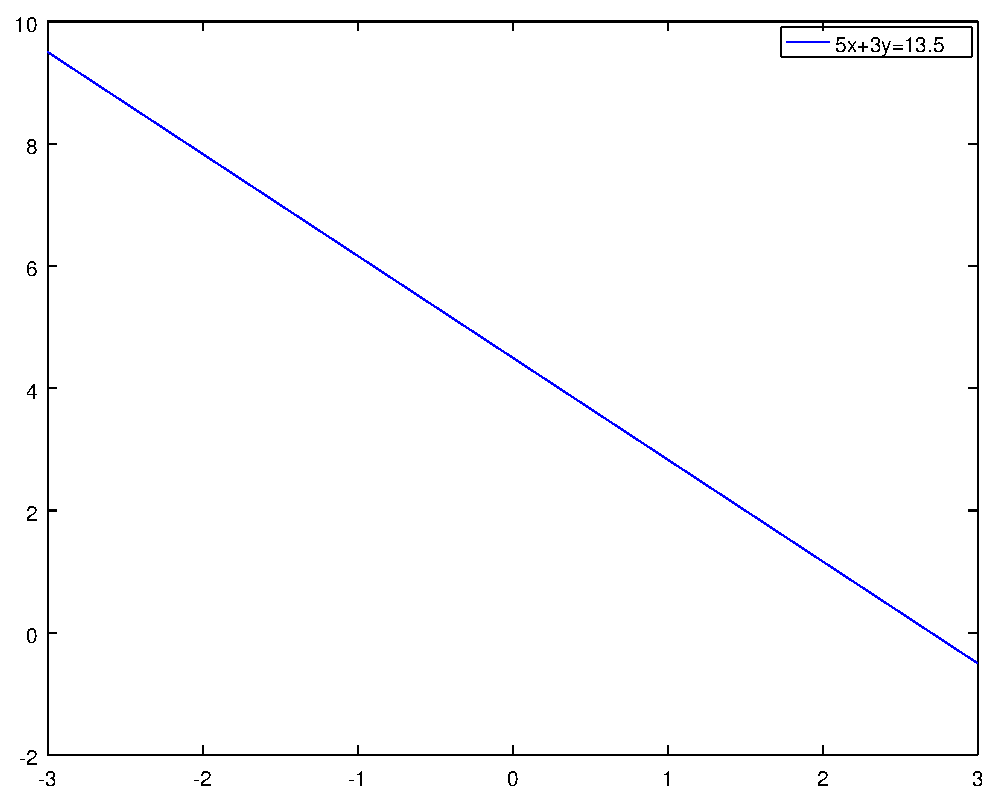
\includegraphics[scale=.6]{./diagrams/gm-03-SystemsEquations-01.eps}
  \end{figure}
\end{frame}

\begin{frame}
  \frametitle{Graphing Method III}
  \begin{figure}[h]
    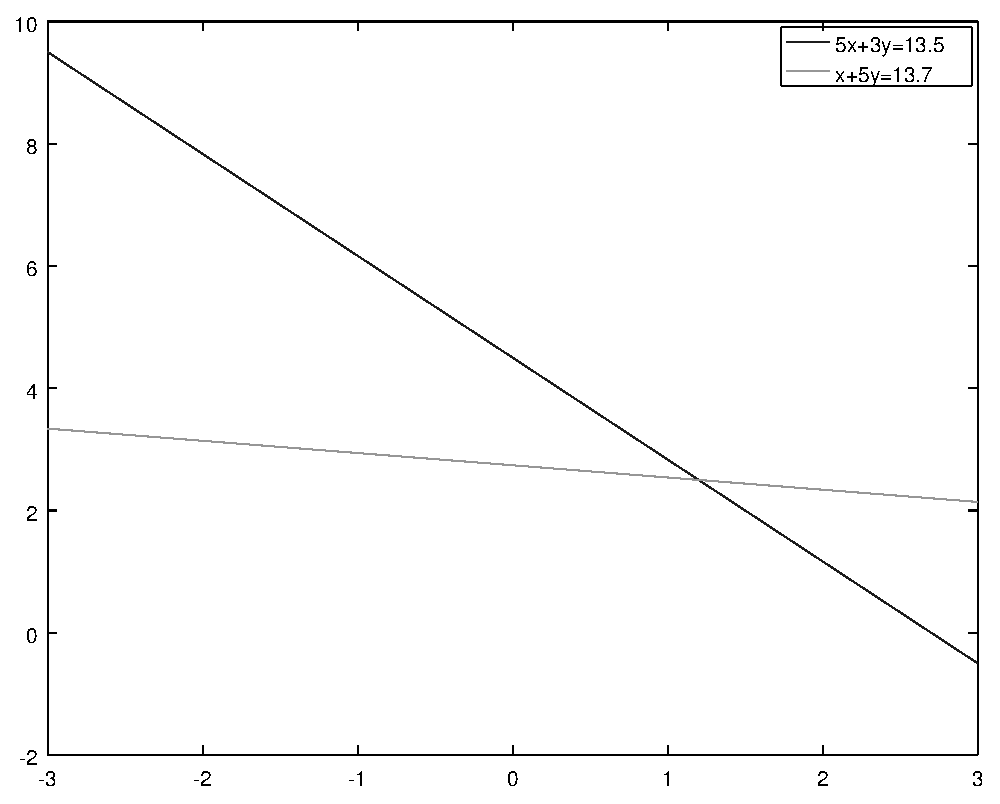
\includegraphics[scale=.6]{./diagrams/gm-03-SystemsEquations-02.eps}
  \end{figure}
\end{frame}

\begin{frame}
  \frametitle{Graphing Method IV}
  \begin{figure}[h]
    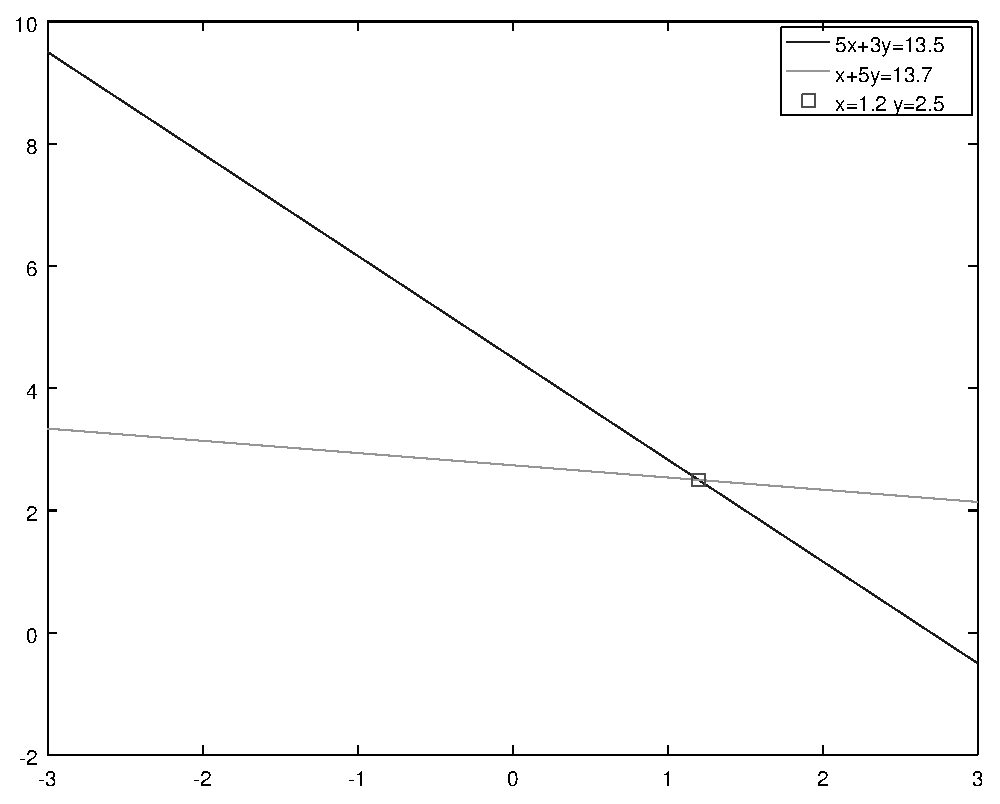
\includegraphics[scale=.6]{./diagrams/gm-03-SystemsEquations-03.eps}
  \end{figure}
\end{frame}

\begin{frame}
  \frametitle{Graphing Method V}
  \begin{figure}[h]
    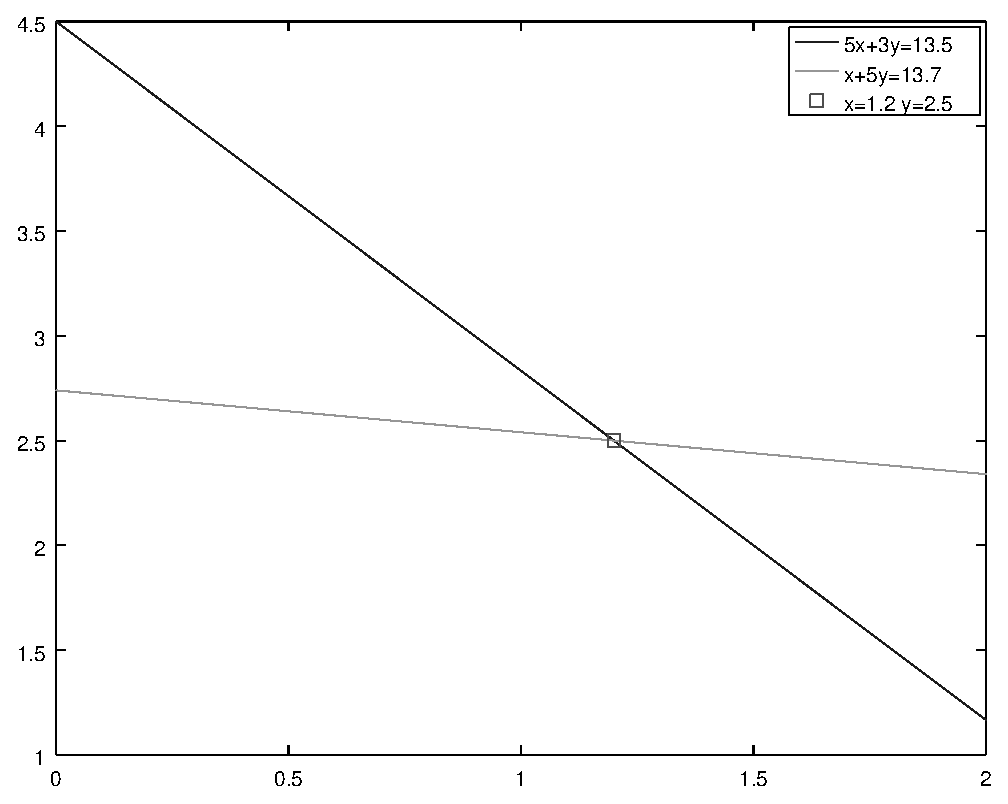
\includegraphics[scale=.6]{./diagrams/gm-03-SystemsEquations-04.eps}
  \end{figure}
\end{frame}

\begin{frame}
  \frametitle{Graphing Method Exercises}
Find a solution to these systems of linear equations by graphing them
and check your answer by substituting.
  \begin{equation}
    \label{eq:fiesebah}
    \begin{array}{rcrcl}
      7x&-&6y&=&19 \\
      -5x&+&2y&=&-9
    \end{array}
  \end{equation}
  \begin{equation}
    \label{eq:weaseiwa}
    \begin{array}{rcrcl}
      x&+&3y&=&12 \\
      11x&-&2y&=&27
    \end{array}
  \end{equation}
  \begin{equation}
    \label{eq:yaetooni}
    \begin{array}{rcrcl}
      \frac{1}{2}x&-&2y&=&\frac{9}{2} \\
      -\frac{5}{8}x&+&y&=&-\frac{15}{8}
    \end{array}
  \end{equation}
\end{frame}

\begin{frame}
  \frametitle{Substitution Method I}
  \begin{equation}
    \label{eq:jichoora}
    \begin{array}{rcrcl}
      5x&+&3y&=&13.5 \\
      x&+&5y&=&13.7
    \end{array}
  \end{equation}
The second equation yields $x=13.7-5y$. Use this to substitute in the
first equation
  \begin{equation}
    \label{eq:iewoobih}
5\cdot\alert{(13.7-5y)}+3y=13.5
  \end{equation}
therefore, $-22y=-55$ and $y=5/2$. Now substitute $y=5/2$ in the first
equation (you could just as well use the second equation), so
\begin{equation}
  \label{eq:phaiyahj}
  5x+3\cdot\frac{5}{2}=13.5
\end{equation}
which implies $x=1.2$. A banana costs \$1.20; an apple costs \$2.50.
\end{frame}

\begin{frame}
  \frametitle{Substitution Method Exercises}
Find a solution to these systems of linear equations by using the
substitution method.
  \begin{equation}
    \label{eq:waduifee}
    \begin{array}{rcrcl}
      7x&-&6y&=&19 \\
      -5x&+&2y&=&-9
    \end{array}
  \end{equation}
  \begin{equation}
    \label{eq:weiyushe}
    \begin{array}{rcrcl}
      x&+&3y&=&12 \\
      11x&-&2y&=&27
    \end{array}
  \end{equation}
  \begin{equation}
    \label{eq:jiadaush}
    \begin{array}{rcrcl}
      \frac{1}{2}x&-&2y&=&\frac{9}{2} \\
      -\frac{5}{8}x&+&y&=&-\frac{15}{8}
    \end{array}
  \end{equation}
\end{frame}

\begin{frame}
  \frametitle{Elimination Method I}
  \begin{equation}
    \label{eq:ohneirae}
    \begin{array}{rcrcl}
      5x&+&3y&=&13.5 \\
      x&+&5y&=&13.7
    \end{array}
  \end{equation}
is equivalent to
  \begin{equation}
    \label{eq:wahheedo}
    \begin{array}{rcrcl}
      5x&+&3y&=&13.5 \\
      5x&+&25y&=&68.5
    \end{array}
  \end{equation}
\end{frame}

\begin{frame}
  \frametitle{Elimination Method II}
  \begin{equation}
    \label{eq:zeegheir}
    \begin{array}{rcrcl}
      5x&+&3y&=&13.5 \\
      5x&+&25y&=&68.5
    \end{array}
  \end{equation}
implies
  \begin{equation}
    \label{eq:ooleeyae}
(5x+3y)-(5x+25y)=13.5-68.5
  \end{equation}
therefore, $-22y=-55$ and $y=5/2$. Now substitute $y=5/2$ in the first
equation (you could just as well use the second equation), so
\begin{equation}
  \label{eq:ieghoisa}
  5x+3\cdot\frac{5}{2}=13.5
\end{equation}
which implies $x=1.2$. A banana costs \$1.20; an apple costs \$2.50.
\end{frame}

\begin{frame}
  \frametitle{Elimination Method Exercises}
Find a solution to these systems of linear equations by using the
elimination method.
  \begin{equation}
    \label{eq:eighilai}
    \begin{array}{rcrcl}
      7x&-&6y&=&19 \\
      -5x&+&2y&=&-9
    \end{array}
  \end{equation}
  \begin{equation}
    \label{eq:thidaitu}
    \begin{array}{rcrcl}
      x&+&3y&=&12 \\
      11x&-&2y&=&27
    \end{array}
  \end{equation}
  \begin{equation}
    \label{eq:ohkaicux}
    \begin{array}{rcrcl}
      \frac{1}{2}x&-&2y&=&\frac{9}{2} \\
      -\frac{5}{8}x&+&y&=&-\frac{15}{8}
    \end{array}
  \end{equation}
\end{frame}

\begin{frame}
  \frametitle{Matrices and Systems of Linear Equations I}
Remember our system of linear equations. 
  \begin{equation}
    \label{eq:ahgohcoh}
    \begin{array}{rcrcl}
      5x & + & 3y & = & 13.5 \\
      x  & + & 5y & = & 13.7
    \end{array}
  \end{equation}
In matrix notation, we can write
  \begin{equation}
    \label{eq:neithohn}
  \left[\begin{array}{cc}
5        & 3                 \\
 1       & 5
  \end{array}\right]\cdot
  \left[\begin{array}{c}
 x                 \\
 y
  \end{array}\right]=
  \left[\begin{array}{c}
13.5                 \\
13.7
  \end{array}\right]\notag
  \end{equation}
\end{frame}

\begin{frame}
  \frametitle{Matrices and Systems of Linear Equations II}
Let's call these three matrices $A,v,b$ respectively. $A$ and $b$ are
provided, and we are looking for $v$. If we had $A^{-1}$, we could go
from
\begin{equation}
  \label{eq:baixieda}
  Av=b
\end{equation}
to
\begin{equation}
  \label{eq:maethung}
  A^{-1}Av=A^{-1}b
\end{equation}
which is the same as
\begin{equation}
  \label{eq:leighuga}
  v=A^{-1}b
\end{equation}
The challenge is therefore to find $A^{-1}$. Scientific calculators
and computers can find $A^{-1}$ for you. 
\end{frame}

\begin{frame}
  \frametitle{Matrix Inverse and Determinants}
  If you want to know how to find the inverse yourself, one method to
  use is calculating the determinant of a matrix. It takes a bit of
  time to understand determinants, and then it's still a complicated
  (and not very transparent) procedure to get to the inverse. For
  $2\times{}2$ matrices, however, the inverse is
  \begin{equation}
    \label{eq:iephaizu}
    A^{-1}=\frac{1}{\det{}A}\left[
      \begin{array}{cc}
        d & -b \\
        -c & a
      \end{array}\right]
  \end{equation}
for
  \begin{equation}
    \label{eq:sooxaexa}
    A=\left[
      \begin{array}{cc}
        a & b \\
        c & d
      \end{array}\right]
  \end{equation}
and the determinant is $\det{}A=ad-bc$.
\end{frame}

\begin{frame}
  \frametitle{Matrix Row Operations}
  Another method to find the inverse of a matrix is using
  \alert{matrix row operations}. There are three matrix row
  operations.
\begin{itemize}
\item \alert{Row Switching} means you are allowed to switch two rows,
  for example $R_{1}\leftrightarrow{}R_{2}$
\item \alert{Row Multiplication} means you are allowed to multiply all
  elements of a row by a real non-zero number, for example
  $\frac{2}{5}R_{2}\rightarrow{}R_{2}$
\item \alert{Row Addition} means you are allowed to add one row to
  another and then replace one of the original rows by the sum of the
  two rows, for example $R_{1}+R_{2}\rightarrow{}R_{1}$
\end{itemize}
Row multiplication and row addition are often used together, for
example $\frac{7}{8}R_{1}-R_{3}\rightarrow{}R_{3}$.
\end{frame}

\begin{frame}
  \frametitle{Matrix Row Operations}
To find the inverse of a square matrix, we combine $A$ and $E$
  \begin{equation}
    \label{eq:aurohbac}
  \left[\begin{array}{cccc}
 5 & 3 & 1 & 0 \\
 1 & 5 & 0 & 1
  \end{array}\right]\notag
  \end{equation}
and apply matrix row operations until we get
  \begin{equation}
    \label{eq:nahshooh}
  \left[\begin{array}{cccc}
 1 & 0 & x & y \\
 0 & 1 & z & w
  \end{array}\right]\notag
  \end{equation}
where
  \begin{equation}
    \label{eq:aecocaeh}
  A^{-1}=\left[\begin{array}{cc}
 x & y  \\
 z & w 
  \end{array}\right]\notag
  \end{equation}
\end{frame}

\begin{frame}
  \frametitle{Inverse Example}
For our example,
  \begin{equation}
    \label{eq:weeraesh}
  \left[\begin{array}{cccc}
 5    & 3     & 1     & 0     \\
 1    & 5     & 0     & 1
  \end{array}\right]\longrightarrow
  \left[\begin{array}{cccc}
 25/3 & 5     & 5/3   & 0     \\
 1    & 5     & 0     & 1
        \end{array}\right]\longrightarrow\notag
\end{equation}
  \begin{equation}
  \left[\begin{array}{cccc}
 22/3 & 0     & 5/3   & -1    \\
 1    & 5     & 0     & 1
  \end{array}\right]\longrightarrow\notag
\end{equation}
  \begin{equation}
    \label{eq:ieyoongu}
  \left[\begin{array}{cccc}
 22/3 & 0     & 5/3   & -1    \\
 22/3 & 110/3 & 0     & 22/3
  \end{array}\right]\longrightarrow
  \left[\begin{array}{cccc}
 22/3 & 0     & 5/3   & -1    \\
 0    & 110/3 & -5/3  & 25/3
  \end{array}\right]\longrightarrow\notag
\end{equation}
  \begin{equation}
    \label{eq:ephoopha}
  \left[\begin{array}{cccc}
 1    & 0     & 5/22  & -3/22 \\
 0    & 1     & -1/22 & 5/22
  \end{array}\right]\notag
  \end{equation}
\end{frame}

\begin{frame}
  \frametitle{Inverse Example}
  For step 1, we multiplied the first row by $5/3$ (row
  multiplication). For step 2, we subtracted the second row from the
  first row and replaced the first row by the result (row addition).
  For step 3, we multiplied the second row by $22/3$ (row
  multiplication). For step 4, we subtracted the first row from the
  second row and replaced the second row by the result (row addition).
  For the last step, we multiplied the first row by $3/22$ and the
  second row by $3/110$ (row multiplication applied twice).
\end{frame}

\begin{frame}
  \frametitle{Matrices and Systems of Linear Equations III}
Thus,
\begin{equation}
  \label{eq:oogeujie}
  A^{-1}=\left[\begin{array}{cc}
 5/22  & -3/22 \\
 -1/22 & 5/22
               \end{array}\right]=\frac{1}{22}\cdot\left[
               \begin{array}{cc}
                 5 & -3 \\
                 -1 & 5
               \end{array}\right]\notag
\end{equation}
and
\begin{equation}
  \label{eq:seeleeje}
  v=A^{-1}b=\left[\begin{array}{cc}
 5/22  & -3/22 \\
 -1/22 & 5/22
  \end{array}\right]\cdot
\left[\begin{array}{c}
 13.5   \\
 13.7  
  \end{array}\right]=\left[\begin{array}{c}
 1.2   \\
 2.5  
  \end{array}\right]\notag
\end{equation}
\end{frame}

\begin{frame}
  \frametitle{End of Lesson}
Next Lesson: Determinants and Inverse
\end{frame}

\end{document}

